% ============================================================
%  Póster: Difusiones y Score
% ============================================================
\documentclass[17pt, a1paper, portrait, margin=0mm, innermargin=12mm,
               blockverticalspace=8mm, colspace=10mm,
               titletotopverticalspace=2mm]{tikzposter}

\usepackage[utf8]{inputenc}
\usepackage[T1]{fontenc}
\usepackage[spanish, es-noshorthands]{babel}
\usepackage{amsmath, amssymb}
\usepackage{graphicx}
\usepackage{tikz}
\usepackage{pgfplots}
\pgfplotsset{compat=1.14}
\usetikzlibrary{arrows.meta, positioning, shapes.geometric, fit}

% ---- Colores propios ----
\definecolor{mainblue}{RGB}{15, 55, 110}
\definecolor{lightblue}{RGB}{210, 225, 245}
\definecolor{accentred}{RGB}{180, 30, 30}
\definecolor{darkgray}{RGB}{60, 60, 60}
\definecolor{blockbg}{RGB}{245, 248, 255}

% ---- Tema ----
\usetheme{Default}
\colorlet{backgroundcolor}{white}
\colorlet{blocktitlebgcolor}{mainblue}
\colorlet{blocktitlefgcolor}{white}
\colorlet{blockbodybgcolor}{blockbg}
\colorlet{blockbodyfgcolor}{black}
\colorlet{titlefgcolor}{mainblue}
\colorlet{titlebgcolor}{white}

% ---- Macros ----
\newcommand{\E}{\mathbb{E}}
\newcommand{\score}{s_\theta}
\newcommand{\dd}{\,\mathrm{d}}

\title{}\author{}\institute{}

\makeatletter
\renewcommand{\TP@maketitle}{%
  \centering
  {\color{titlefgcolor}
    {\bfseries\Huge\sc Difusiones y Score\par}%
    \vspace{0.15em}%
    {\Large La matem\'atica detr\'as de los modelos generativos modernos\par}%
    \vspace{0.25em}%
    {\huge Gonzalo Josu\'e Spina\par}%
    \vspace{0.15em}%
    {\large Universidad de Buenos Aires \textbullet\
      Facultad de Ciencias Exactas y Naturales \textbullet\
      C\'alculo Estoc\'astico, 2026}%
  }%
}
\makeatother

\begin{document}
\maketitle

\begin{columns}

%%% ─── COLUMNA IZQUIERDA (0.30) ──────────────────────────────
\column{0.30}

\block{1. El problema}{
\begin{center}
\begin{tikzpicture}[scale=0.95]
\foreach \x/\y in {
  0.2/1.2, 0.6/0.9, 0.9/1.4, 1.2/0.8, 1.4/1.1,
  0.4/1.7, 0.8/1.5, 1.1/1.8, 1.5/1.6, 0.3/2.1,
  0.7/2.3, 1.0/2.0, 1.4/2.2, 0.5/0.5, 1.1/0.4}{
  \fill[mainblue, opacity=0.75] (\x,\y) circle (6pt);
}
\foreach \x/\y in {
  2.8/1.0, 3.2/0.7, 3.5/1.2, 3.8/0.9, 3.1/1.5,
  2.6/1.8, 3.0/2.0, 3.4/1.7, 3.7/2.1, 2.9/2.4,
  3.3/2.3, 3.8/1.4, 2.5/1.1, 3.6/0.5, 3.1/0.4}{
  \fill[mainblue!55, opacity=0.75] (\x,\y) circle (6pt);
}
\node[darkgray, font=\normalsize] at (2.0,-0.35)
  {Muestras de $p_0(x)$ (desconocida)};
\end{tikzpicture}
\end{center}

\bigskip
\textbf{Queremos} generar nuevas muestras de $p_0(x)$.

\medskip
\textbf{Problema:} $p_0(x)$ es desconocida; solo tenemos datos.

\medskip
\emph{Idea:} corromper los datos con ruido hasta llegar a una
distribuci\'on \textbf{conocida} $\pi$; luego invertir el proceso.
}

\block{2. Difusiones como modelos generativos}{
Definimos un proceso estoc\'astico \textbf{forward} que transforma
$p_0$ gradualmente en una distribuci\'on conocida $\pi$:
\[
  \dd X_t = f(X_t,t)\,\dd t + g(t)\,\dd B_t,
  \qquad X_0 \sim p_0.
\]
Dise\~nando $f$ y $g$ para que $p_T \approx \pi$ (e.g.\ gaussiana),
obtenemos un proceso que \emph{destruye} la estructura de los datos.

\medskip
\textbf{Resultado clave (Anderson, 1982).}
El proceso corriendo en tiempo inverso $\tau = T - t$
es tambi\'en una difusi\'on, con la \textbf{misma estructura}
que el forward m\'as un t\'ermino adicional: el \textbf{score}.
}

\block{3. Proceso forward: Ornstein-Uhlenbeck}{
Difundimos los datos con el \textbf{proceso OU}
($f(x,t) = -x$, $g = \sigma$):
\[
  \dd X_t = -X_t\,\dd t + \sigma\,\dd B_t, \qquad X_0 \sim p_0.
\]
La soluci\'on desde $X_0 = x_0$ es:
\[
  X_t \mid x_0 \;\sim\;
  \mathcal{N}\!\Bigl(x_0\,e^{-t},\;\tfrac{\sigma^2}{2}(1-e^{-2t})\Bigr).
\]
El autovalor $\lambda = -1 < 0$ del drift garantiza convergencia
(al igual que en $\dot{x} = -x$), y para $T$ grande
$p_T \approx \mathcal{N}(0,\,\sigma^2/2)$.

\begin{center}
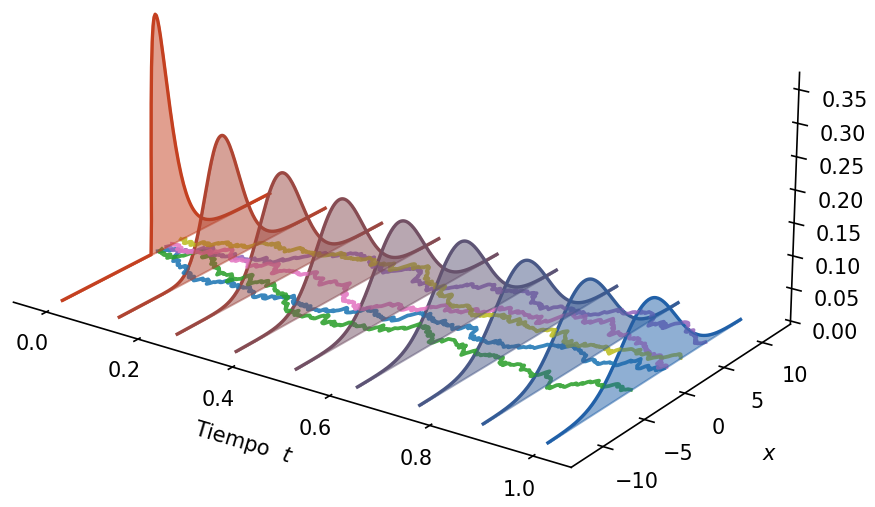
\includegraphics[width=0.97\linewidth]{fig1_forward.png}
\end{center}
}

%%% ─── COLUMNA CENTRAL (0.43) ────────────────────────────────
\column{0.43}

\block{4. Anderson (1982): caso OU}{
\[
  \dd \hat{X}_\tau
  = \Bigl[\hat{X}_\tau + \sigma^2\,{\color{accentred}\nabla_x \log p_{T-\tau}}\Bigr]\dd\tau
  + \sigma\,\dd\bar{B}_\tau.
\]

\begin{center}
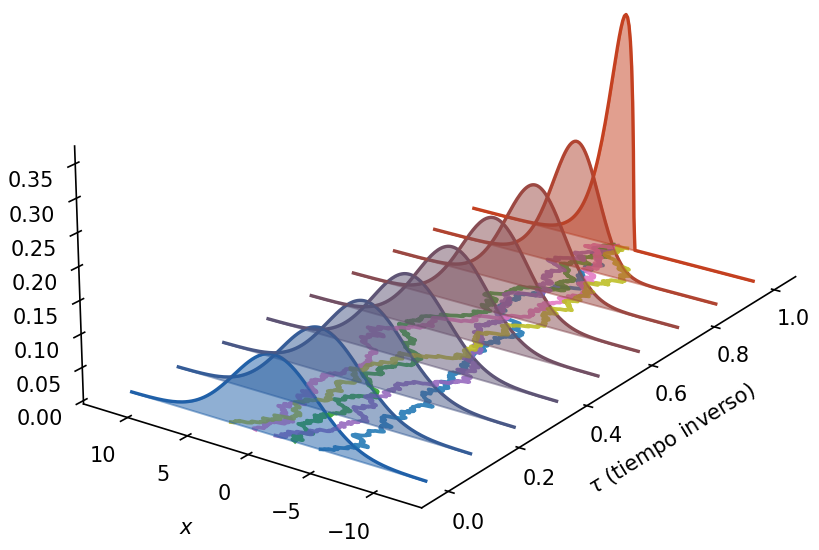
\includegraphics[width=0.97\linewidth]{fig3_reverse_sde.png}
\end{center}
}

\block{5. El score: qu\'e es y qu\'e hace}{
El ingrediente desconocido
${\color{accentred}\nabla_x \log p_t(x)}$ se llama \textbf{score}.
Es el gradiente del logaritmo de la densidad:
apunta hacia las regiones de mayor probabilidad
y es el motor que impulsa el proceso inverso.

\medskip
El campo vectorial muestra c\'omo var\'ia con $t$ y $x$
(de Gamma a Gaussiana).
Las trayectorias negras son part\'iculas guiadas por el score.

\begin{center}
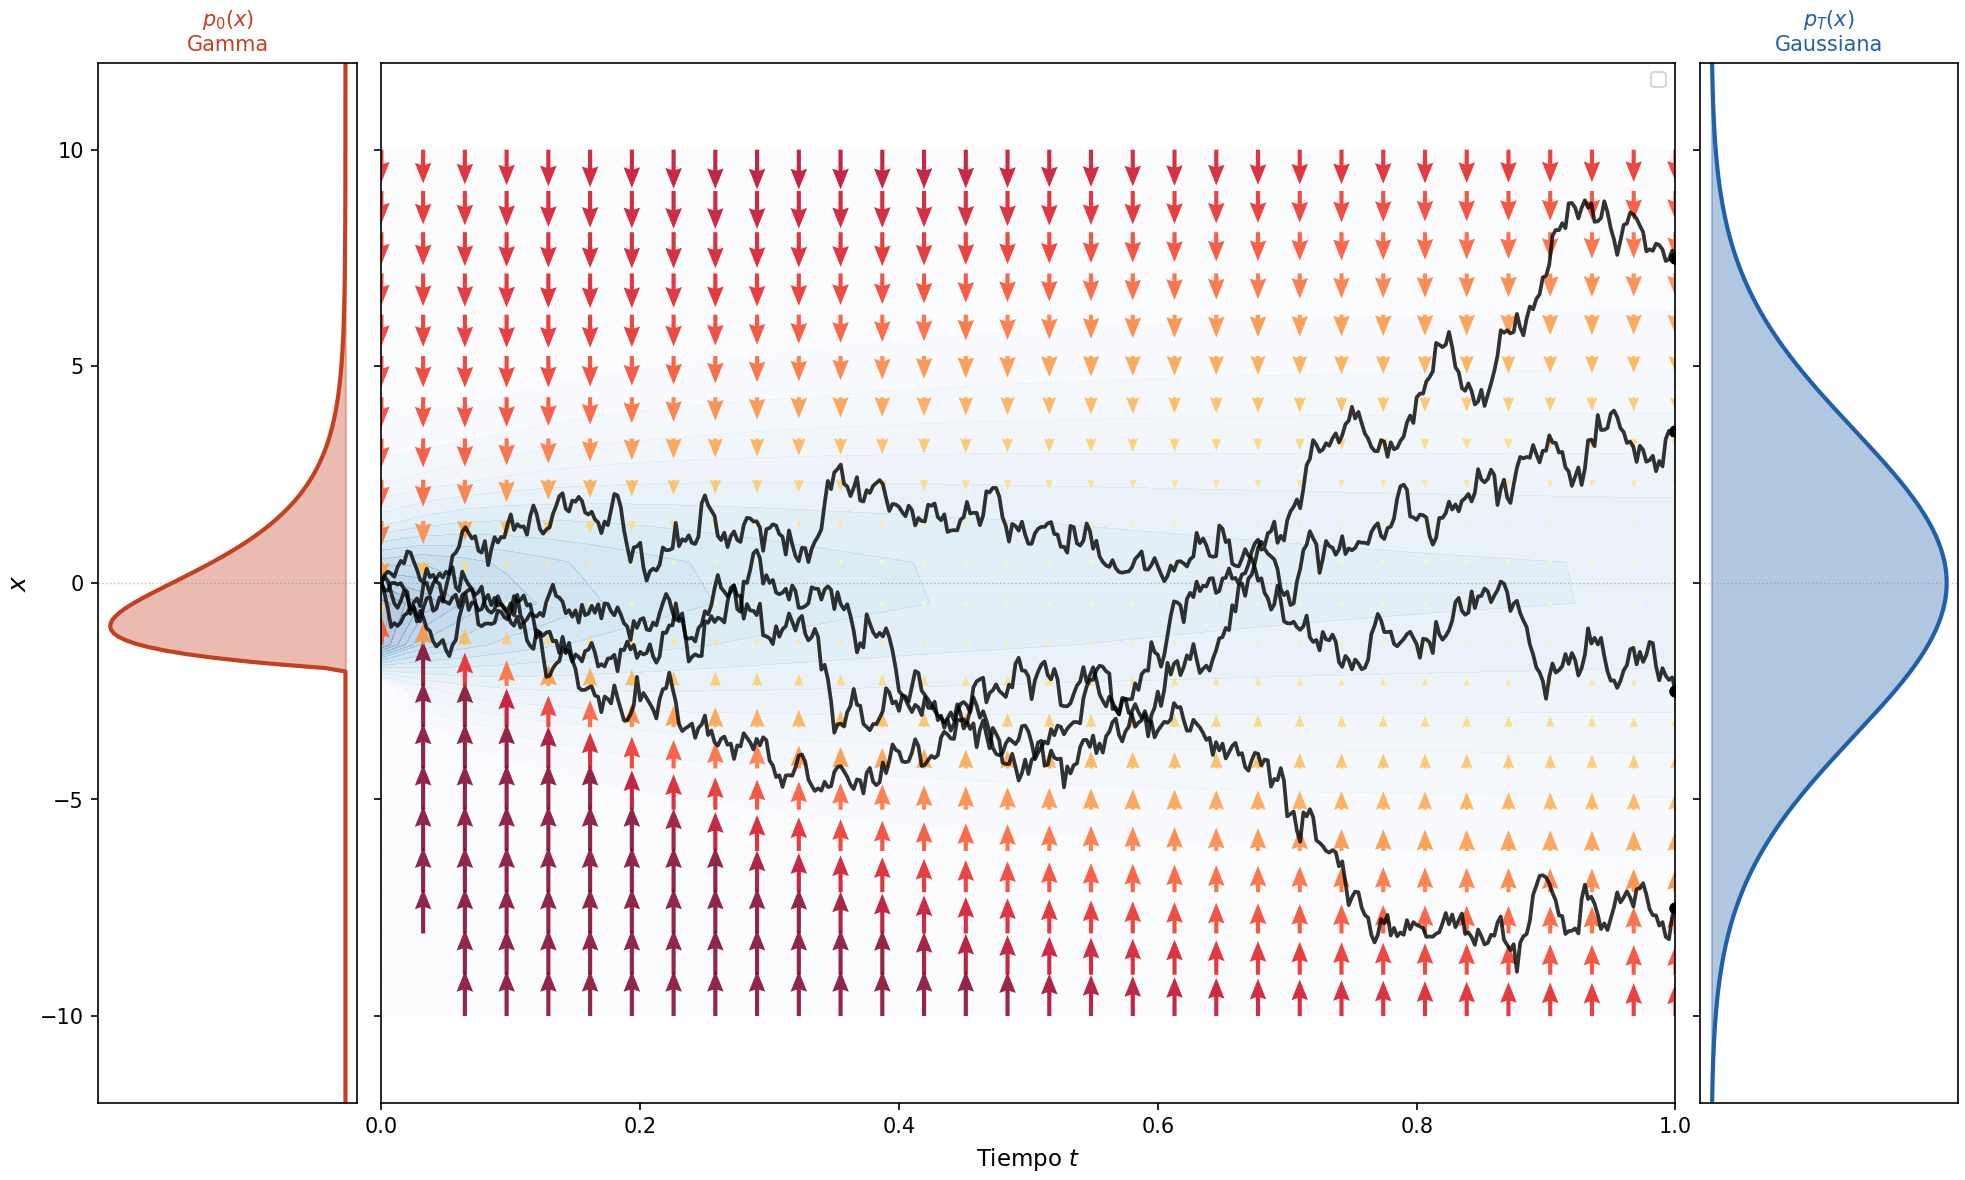
\includegraphics[width=0.97\linewidth]{fig2_score.png}
\end{center}

\emph{Objetivo:} aprender $\score(x,t) \approx \nabla_x \log p_t(x)$.
}

\block{6. C\'omo aprender el score}{
\textbf{Hyv\"arinen (2005).} El objetivo natural es intratable
porque requiere $\nabla_x \log p$:
\[
  J_{\text{nat}}(\theta)
  = \tfrac{1}{2}\,\E\bigl[\|\score(x) - \nabla_x \log p(x)\|^2\bigr].
\]
Integrando por partes se elimina ese t\'ermino:
\[
  J(\theta)
  = \E\!\left[
      \operatorname{tr}\!\bigl(\nabla_x \score(x)\bigr)
      + \tfrac{1}{2}\,\|\score(x)\|^2
    \right] + \text{cte.}
\]

\medskip\rule{\linewidth}{0.5pt}\medskip

\textbf{Vincent (2011).}
Consideremos la marginal ruidosa
$p_\sigma(\tilde{x}) = \int q_\sigma(\tilde{x}\!\mid\! x)\,p_0(x)\,\dd x$
con $q_\sigma(\tilde{x}\!\mid\! x) = \mathcal{N}(x,\sigma^2 I)$.
Diferenciando bajo la integral se obtiene la identidad de score:
\[
  \nabla_{\tilde{x}} \log p_\sigma(\tilde{x})
  = \E_x\!\Bigl[\nabla_{\tilde{x}} \log q_\sigma(\tilde{x}\!\mid\! x)
    \;\Big|\; \tilde{x}\Bigr].
\]
El score de la \textbf{marginal} (desconocido) es la esperanza del
score de la \textbf{condicional} (conocido):
\[
  \nabla_{\tilde{x}}\log q_\sigma(\tilde{x}\mid x)
  = -\frac{\tilde{x}-x}{\sigma^2}.
\]
Minimizar sobre la condicional es equivalente a minimizar sobre la
marginal, lo que da el objetivo pr\'actico:
\[
  \tilde{J}(\theta)
  = \E\!\left[
      \Bigl\|\score(\tilde{x},\sigma)
        + \frac{\tilde{x}-x}{\sigma^2}\Bigr\|^2
    \right].
\]
}

%%% ─── COLUMNA DERECHA (0.27) ────────────────────────────────
\column{0.27}

\block{7. \textquestiondown Qu\'e aprende la red?}{
\begin{center}
\begin{tikzpicture}[
  node distance=14mm,
  box/.style={draw=mainblue, fill=lightblue!50, rounded corners=5pt,
              minimum width=65mm, minimum height=15mm,
              font=\normalsize, align=center},
  redbox/.style={draw=accentred, fill=accentred!10, rounded corners=5pt,
                 minimum width=65mm, minimum height=15mm,
                 font=\normalsize\bfseries, align=center},
  graybox/.style={draw=darkgray, fill=gray!12, rounded corners=5pt,
                  minimum width=65mm, minimum height=15mm,
                  font=\normalsize, align=center},
  arr/.style={-{Stealth}, mainblue, line width=2pt},
  lbl/.style={font=\small\itshape, darkgray}
]
\node[box]     (x)   {$x \sim p_0$};
\node[box,     below=of x]   (xn)  {$\tilde{x} = x + \sigma\varepsilon$};
\node[redbox,  below=of xn]  (net) {FFN / U-Net};
\node[box,     below=of net] (out) {$\hat{s}_\theta(\tilde{x},\,\sigma)$};
\node[graybox, below=of out] (tgt) {Target: $-(\tilde{x}-x)/\sigma^2$};

\draw[arr] (x)   -- (xn)  node[midway, right=3mm, lbl] {ruido $\sigma\varepsilon$};
\draw[arr] (xn)  -- (net);
\draw[arr] (net) -- (out);
\draw[-{Stealth}, darkgray, dashed, line width=1.5pt]
  (tgt) -- (out) node[midway, right=3mm, lbl] {supervisi\'on};
\end{tikzpicture}
\end{center}

\medskip
\begin{center}
\emph{La red nunca aprende una densidad.}\\[4pt]
Aprende un \textbf{campo vectorial} $x \mapsto \hat{s}_\theta(x,t)$.
\end{center}
}

\subcolumn{0.49}

\block{8. Probability flow ODE}{
El proceso inverso \textbf{no necesita ser ruidoso}.
Existe una ODE determinista con las mismas marginales $p_t$:
\[
  \dd \hat{X}_\tau
  = \Bigl[\hat{X}_\tau
    + \tfrac{\sigma^2}{2}\,{\color{accentred}\nabla_x \log p_{T-\tau}}\Bigr]\dd\tau.
\]

\begin{center}
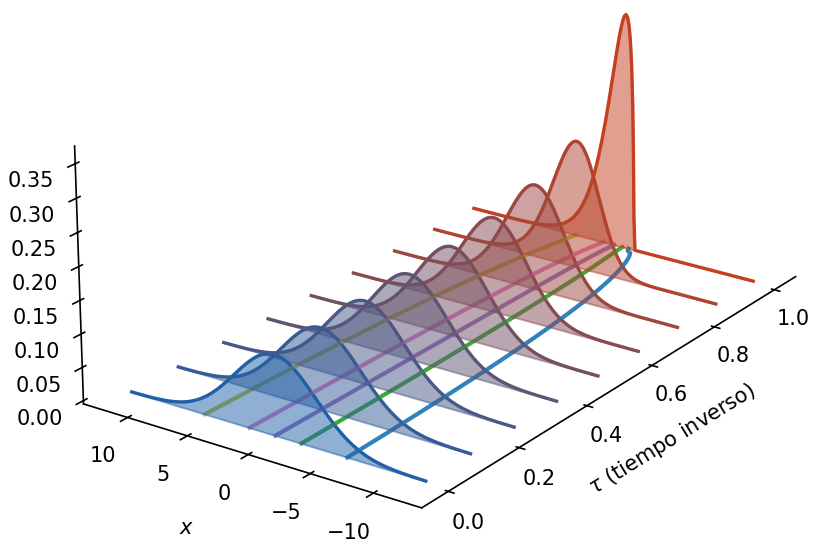
\includegraphics[width=0.97\linewidth]{fig4_pflow.png}
\end{center}

Dado $x_T$, el camino hacia $x_0$ es \textbf{determinista y \'unico}.
}

\block{9. Cierre: el pipeline funciona}{
\textbf{Pipeline de generaci\'on:}
\begin{enumerate}\itemsep1pt
  \item Muestrear $\hat{X}_T \sim \mathcal{N}(0,\,\sigma^2/2)$
  \item Correr la EDE inversa (o la ODE) de $T$ a $0$
  \item Obtener $\hat{X}_0 \sim p_0$
\end{enumerate}

Con el score aprendido v\'ia denoising score matching,
la EDE inversa recupera muestras de $p_0$
partiendo de $\mathcal{N}(0,\,\sigma^2/2)$:

\begin{center}
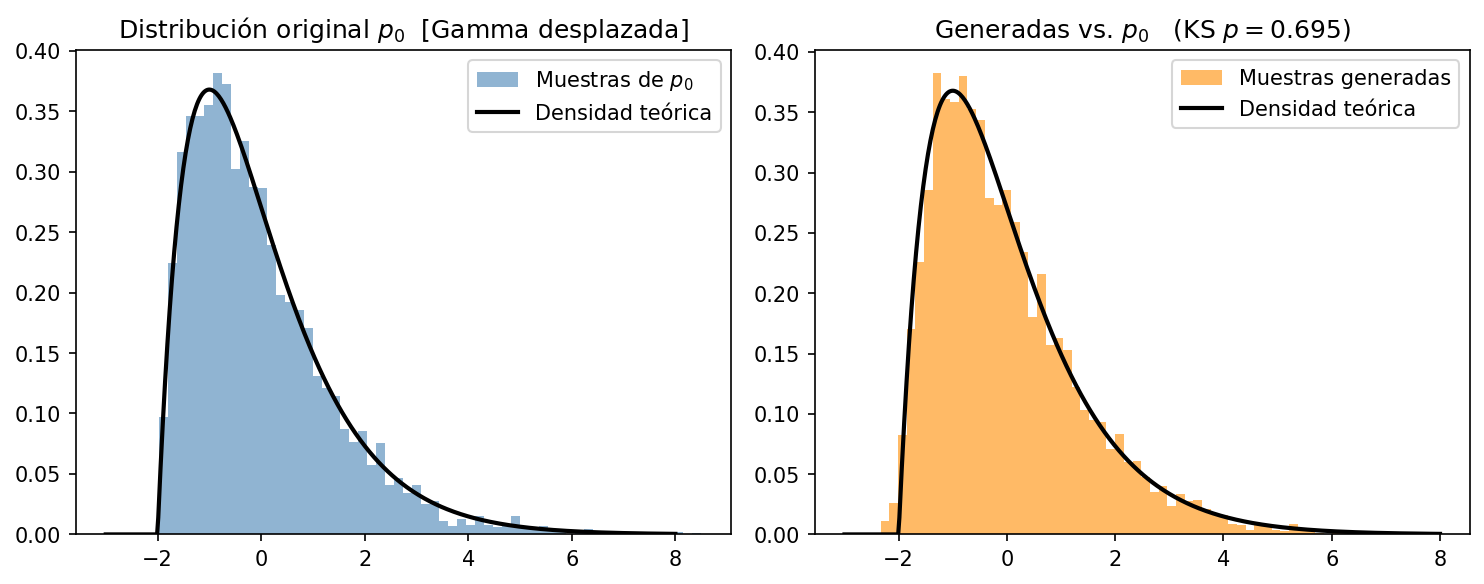
\includegraphics[width=0.90\linewidth]{score_matching_demo.png}
\end{center}

\begin{center}
{\color{mainblue}
Test KS: $p = 0.695$ --- no se rechaza $H_0\colon \hat{p} = p_0$.\\[4pt]
\textbf{Geometr\'ia $+$ probabilidad $+$ aprendizaje profundo.}}
\end{center}
}

\end{columns}
\end{document}
